%%%%%%%%%%%%%%%%%%%%%%%%%%%%%%%%%%%%%%%%%
% Stylish Article
% LaTeX Template
% Version 2.2 (2020-10-22)
%
% This template has been downloaded from:
% http://www.LaTeXTemplates.com
%
% Original author:
% Mathias Legrand (legrand.mathias@gmail.com) 
% With extensive modifications by:
% Vel (vel@latextemplates.com)
% Jacqueline Näther (jnaether@uni-osnabrueck.com)
% Fabian Imkenberg (fimkenberg@uni-osnabrueck.com)
%
% License:
% CC BY-NC-SA 3.0 (http://creativecommons.org/licenses/by-nc-sa/3.0/)
%
%%%%%%%%%%%%%%%%%%%%%%%%%%%%%%%%%%%%%%%%%

%----------------------------------------------------------------------------------------
%	PACKAGES AND OTHER DOCUMENT CONFIGURATIONS
%----------------------------------------------------------------------------------------

\documentclass[fleqn,10pt]{SelfArx} % Document font size and equations flushed left

\usepackage[english]{babel} % Specify a different language here - english by default

\usepackage{lipsum} % Required to insert dummy text. To be removed otherwise

%----------------------------------------------------------------------------------------
%	COLUMNS
%----------------------------------------------------------------------------------------

\setlength{\columnsep}{0.55cm} % Distance between the two columns of text
\setlength{\fboxrule}{0.75pt} % Width of the border around the abstract

%----------------------------------------------------------------------------------------
%	COLORS
%----------------------------------------------------------------------------------------

\definecolor{color1}{RGB}{172,06,52} % Corporate Design Colour of University of Osnabrueck
\definecolor{color2}{RGB}{207,208,209} % Corporate Design Colour of University of Osnabrueck
\definecolor{color3}{RGB}{251,185,0} % Corporate Design Colour of University of Osnabrueck

%----------------------------------------------------------------------------------------
%	HYPERLINKS
%----------------------------------------------------------------------------------------

\usepackage{hyperref} % Required for hyperlinks

\hypersetup{
	hidelinks,
	colorlinks,
	breaklinks=true,
	urlcolor=color3,
	citecolor=color1,
	linkcolor=color1,
	bookmarksopen=false,
	pdftitle={Title},
	pdfauthor={Author},
}

%----------------------------------------------------------------------------------------
%	ARTICLE INFORMATION
%----------------------------------------------------------------------------------------

\JournalInfo{
\includegraphics[width=0.3\linewidth]{logo_uni}}
\Archive{} %!!NEEDED, otherwise \tableofcontent error, is for Additional notes below university logo (e.g. copyright, DOI, review/research article)

\PaperTitle{Reimplementation of a Cycle-Consistent Adversarial Network for unpaired Image-to-Image Translation}

\Authors{Fabian Imkenberg, Jacqueline Naether}

\Keywords{CycleGAN --- Keyword2 --- Keyword3} 
\newcommand{\keywordname}{Keywords} % Defines the keywords heading name

%----------------------------------------------------------------------------------------
%	ABSTRACT
%----------------------------------------------------------------------------------------

\Abstract{Lorem ipsum dolor sit amet, consectetuer adipiscing elit. Ut purus elit, vestibulum ut, placerat ac, adipiscing vitae, felis. Curabitur dictum gravida mauris. Nam arcu libero, nonummy eget, consectetuer id, vulputate a, magna. Donec vehicula augue eu neque. Pellentesque habitant morbi tristique senectus et netus et malesuada fames ac turpis egestas. Mauris ut leo. Cras viverra metus rhoncus sem. Nulla et lectus vestibulum urna fringilla ultrices. Phasellus eu tellus sit amet tortor gravida placerat. Integer sapien est, iaculis in, pretium quis, viverra ac, nunc. Praesent eget sem vel leo ultrices bibendum. Aenean faucibus. Morbi dolor nulla, malesuada eu, pulvinar at, mollis ac, nulla. Curabitur auctor semper nulla. Donec varius orci eget risus. Duis nibh mi, congue eu, accumsan eleifend, sagittis quis, diam. Duis eget orci sit amet orci dignissim rutrum.}

%----------------------------------------------------------------------------------------

\begin{document}
\maketitle
\tableofcontents
\thispagestyle{empty} % Removes page numbering from the first page

%----------------------------------------------------------------------------------------
%	ARTICLE CONTENTS
%----------------------------------------------------------------------------------------

\section*{Introduction}
\addcontentsline{toc}{section}{Introduction}
Wir benutzen die Paper \cite{image-to-image-can} und \cite{image-to-image-ccan}.
\lipsum[1-3] % Dummy text
 and some mathematics $\cos\pi=-1$ and $\alpha$ in the text\footnote{And some mathematics $\cos\pi=-1$ and $\alpha$ in the text.}.

%------------------------------------------------

\section{Methods}

\begin{figure*}[ht]\centering % Using \begin{figure*} makes the figure take up the entire width of the page
	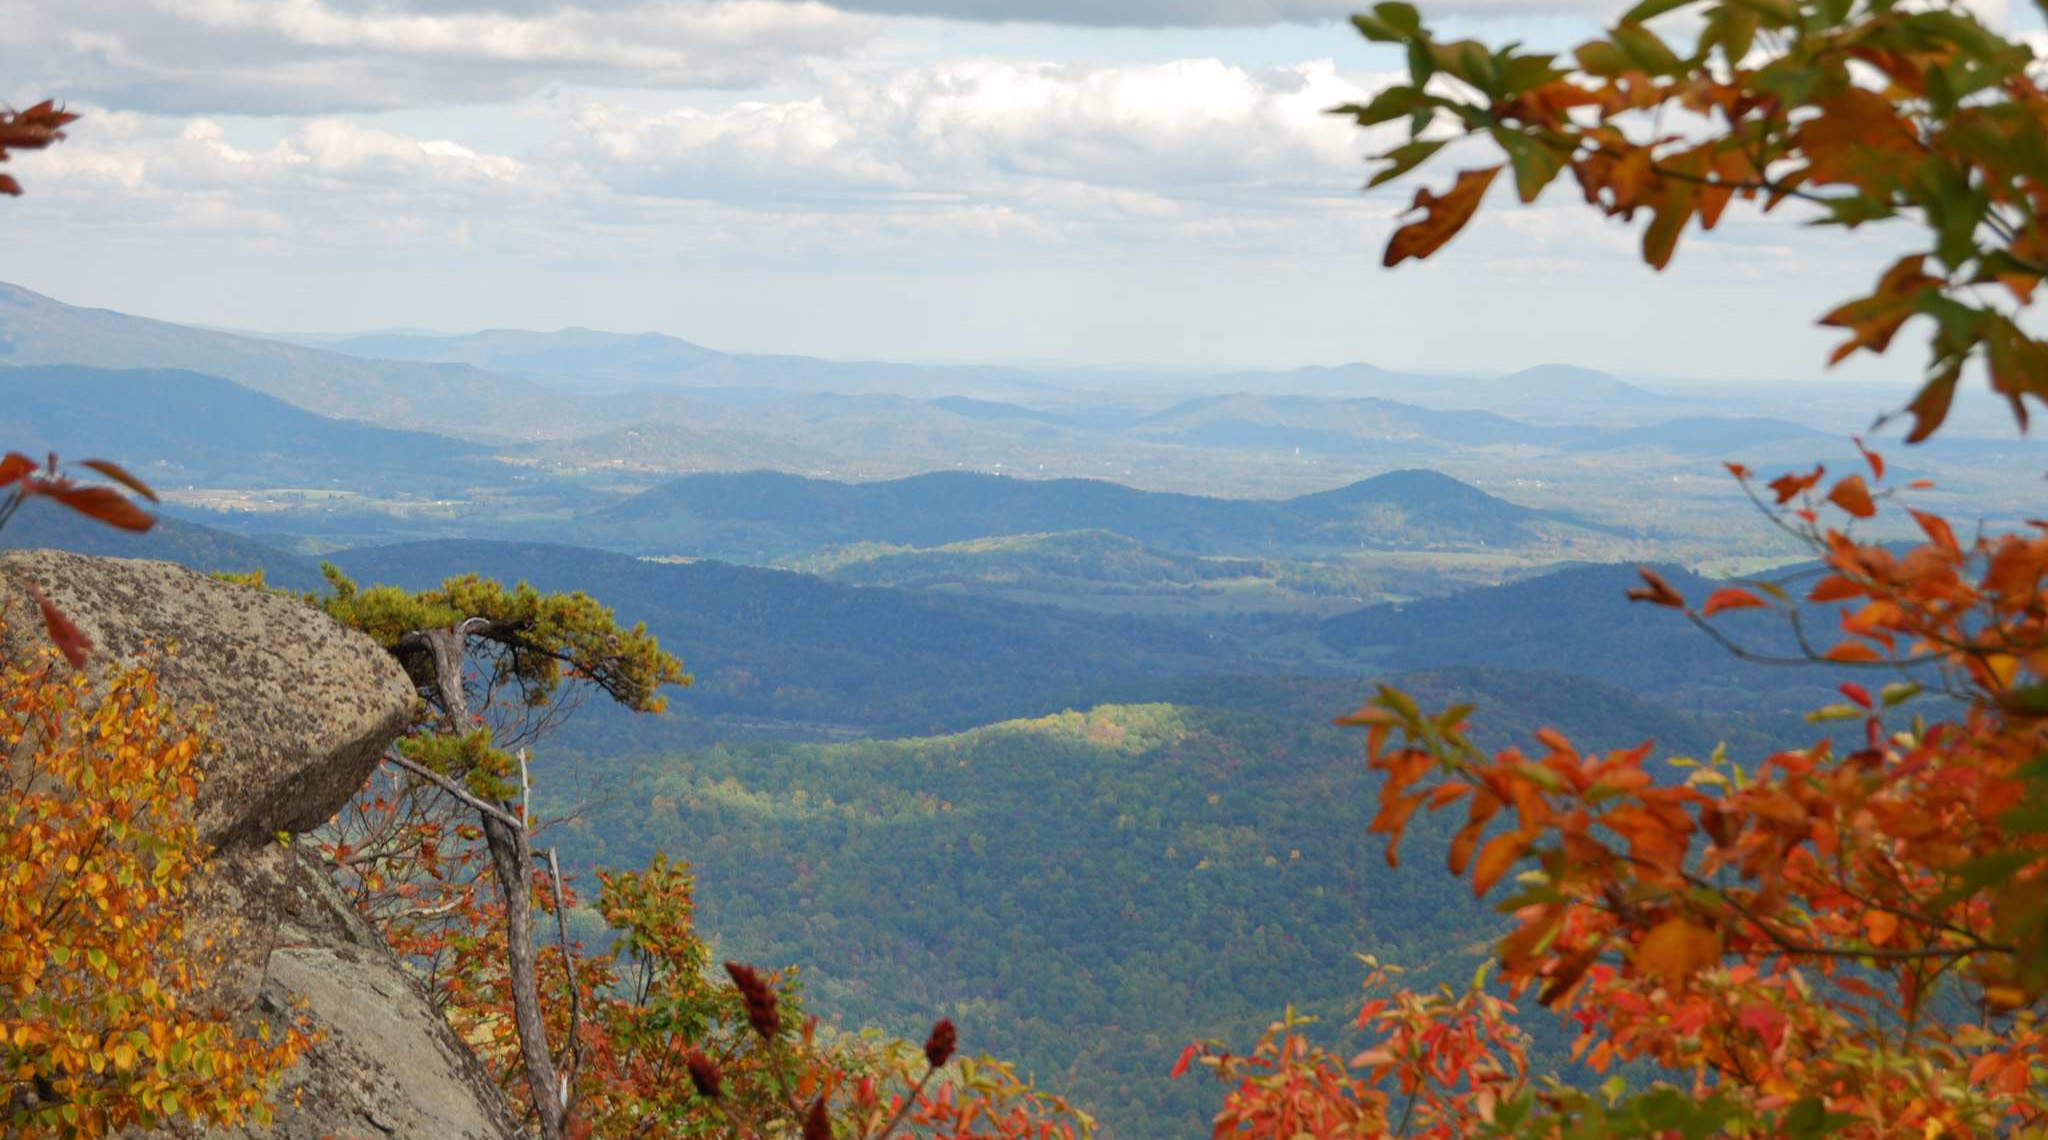
\includegraphics[width=\linewidth]{view}
	\caption{Wide Picture}
	\label{fig:view}
\end{figure*}

\lipsum[2] % Dummy text

\begin{equation}
	\cos^3 \theta =\frac{1}{4}\cos\theta+\frac{3}{4}\cos 3\theta
	\label{eq:refname2}
\end{equation}

\lipsum[2] % Dummy text

\begin{enumerate}[noitemsep] % [noitemsep] removes whitespace between the items for a compact look
	\item First item in a list
	\item Second item in a list
	\item Third item in a list
\end{enumerate}

\subsection{Network Architecture}

\lipsum[3] % Dummy text

\paragraph{GAN} \lipsum[2] % Dummy text
\paragraph{CycleGAN} \lipsum[2] % Dummy text

\subsection{Formulation}

\lipsum[4] % Dummy text
\paragraph{Adversarial Loss} \lipsum[2] % Dummy text
\paragraph{Cycle Consistency Loss} \lipsum[2] % Dummy text

\begin{figure}[ht]\centering
	\includegraphics[width=\linewidth]{results}
	\caption{In-text Picture}
	\label{fig:results}
\end{figure}

Reference to Figure \ref{fig:results}.

%------------------------------------------------
\section{Implementation}
\lipsum[9] % Dummy text
\subsection{Pre-Processing} \lipsum[2] % Dummy text
\subsection{Training} \lipsum[2] % Dummy text
\subsection{Test} \lipsum[2] % Dummy text

%------------------------------------------------

\section{Results}

\lipsum[3] % Dummy text

\subsection{Evaluation}

\lipsum[3] % Dummy text

\begin{table}[hbt]
	\caption{Table of Grades}
	\centering
	\begin{tabular}{llr}
		\toprule
		\multicolumn{2}{c}{Name} \\
		\cmidrule(r){1-2}
		First name & Last Name & Grade \\
		\midrule
		John & Doe & $7.5$ \\
		Richard & Miles & $2$ \\
		\bottomrule
	\end{tabular}
	\label{tab:label}
\end{table}


\subsection{Subsection}

\lipsum[6] % Dummy text

%------------------------------------------------

\section{Limitations and Discussion}

\lipsum[5] % Dummy text
%----------------------------------------------------------------------------------------
%	REFERENCE LIST
%----------------------------------------------------------------------------------------

\phantomsection
\bibliographystyle{unsrt}
\bibliography{sample.bib}

%----------------------------------------------------------------------------------------

\end{document}